\section{Diseño arquitectónico}

El sistema es un gestor de base de datos escrito desde cero en Python. \textbf{Ninguna
estructura evaluada se delega en una librería}: las páginas, los árboles, el hash, los
algoritmos externos, el parser y el índice espacial están implementados a mano. Las
dependencias externas se limitan a lo que el enunciado no evalúa: el servidor web
(FastAPI), la interfaz (React, Leaflet), las gráficas y las pruebas.

\begin{center}
\begin{tikzpicture}[
  capa/.style={draw=acento, fill=acentoSuave, rounded corners=2pt, minimum height=6.2mm,
               minimum width=9.6cm, font=\footnotesize},
  base/.style={draw=exito, fill=exitoSuave, rounded corners=2pt, minimum height=6.2mm,
               minimum width=9.6cm, font=\footnotesize},
  nota/.style={font=\scriptsize\itshape, color=gris, anchor=west},
  node distance=1.4mm]
  \node[capa] (ui)  {\texttt{frontend/} \quad React, TypeScript, Leaflet};
  \node[capa, below=of ui]  (api) {\texttt{api/} \quad REST (FastAPI), una sesión por pestaña};
  \node[capa, below=of api] (txn) {\texttt{txn/} \quad sesiones, bloqueos en dos fases, deshacer};
  \node[capa, below=of txn] (qry) {\texttt{sql/} + \texttt{query/} \quad parser, catálogo,
                                   planificador, operadores};
  \node[capa, below=of qry] (idx) {\texttt{index/} \quad B+ agrupado y no agrupado, hash
                                   extendible, R-Tree};
  \node[capa, below=of idx] (ext) {\texttt{external/} \quad ordenamiento, hashing y bucles
                                   anidados externos};
  \node[base, below=of ext] (sto) {\texttt{storage/} \quad registros, páginas, buffer pool,
                                   heap, secuencial};
  \node[base, below=of sto] (spa) {\texttt{spatial/} \quad geometría y métricas (sin
                                   dependencias)};
  \node[nota] at ([xshift=2mm]ui.east)  {HTTP};
  \node[nota] at ([xshift=2mm]txn.east) {aislamiento};
  \node[nota] at ([xshift=2mm]qry.east) {de SQL a filas};
  \node[nota] at ([xshift=2mm]idx.east) {caminos de acceso};
  \node[nota] at ([xshift=2mm]sto.east) {bytes en disco};
\end{tikzpicture}
\end{center}

\textbf{Cada capa solo conoce a la de abajo}: el motor no sabe qué es una transacción ni
que existe un API, y el API no sabe nada de la interfaz. Cuatro decisiones atraviesan todas
las capas:

\begin{itemize}[nosep, leftmargin=*]
  \item \textbf{Todo opera por páginas.} Ninguna estructura abre archivos por su cuenta:
        piden páginas de 4\,096 bytes a un único paginador, con un \emph{buffer pool} LRU
        de 128 páginas. Nada carga un archivo entero en memoria.
  \item \textbf{Registros de tamaño fijo.} La posición de un registro en su página es una
        multiplicación, no una búsqueda; la capacidad de un nodo se \emph{deduce} de dividir
        el tamaño de página entre el de una entrada.
  \item \textbf{Una sola implementación de cada cosa.} La serialización, el manejo de
        páginas y las métricas de distancia viven en un único lugar: una consulta no puede
        dar resultados distintos según el camino que elija el planificador.
  \item \textbf{Nada incrustado.} Tamaño de página, umbrales, abanicos y particiones son
        campos de \texttt{EngineConfig}; rutas y direcciones, variables de entorno; los
        parámetros de los experimentos, argumentos de línea de comandos.
\end{itemize}

\paragraph{El camino de una consulta.} Toda sentencia recorre la misma cadena, y su
resultado lleva, además de las filas, el \textbf{plan de ejecución} con el camino de acceso
elegido y ---con \texttt{EXPLAIN ANALYZE}--- las filas y el tiempo de cada operador.

\begin{center}
\begin{tikzpicture}[
  paso/.style={draw=acento, fill=acentoSuave, rounded corners=2pt, minimum height=7mm,
               font=\scriptsize, align=center, inner sep=3pt},
  node distance=3.5mm]
  \node[paso] (a) {texto\\SQL};
  \node[paso, right=of a] (b) {lexer\\tokens};
  \node[paso, right=of b] (c) {parser\\AST};
  \node[paso, right=of c] (d) {validación\\de tipos};
  \node[paso, right=of d] (e) {planificador\\camino de acceso};
  \node[paso, right=of e] (f) {operadores\\(iteradores)};
  \node[paso, right=of f] (g) {filas\\+ plan};
  \foreach \x/\y in {a/b, b/c, c/d, d/e, e/f, f/g} \draw[flecha] (\x) -- (\y);
\end{tikzpicture}
\end{center}

\paragraph{API e interfaz.} El API expone el motor sin lógica propia: ejecuta guiones SQL,
lista el catálogo, describe la estructura física de una tabla y de sus índices, y crea
tablas a partir de un CSV. Cada pestaña del navegador es una sesión, de modo que dos
pestañas bastan para demostrar bloqueos. La interfaz (figura~\ref{fig:interfaz}) muestra a
la vez los cuatro paneles del enunciado ---archivos, consultas, resultados y plan--- y,
para la Parte~2, un mapa con el resultado, la figura de la consulta y los MBR del R-Tree.

\begin{figure}[!htb]
  \centering
  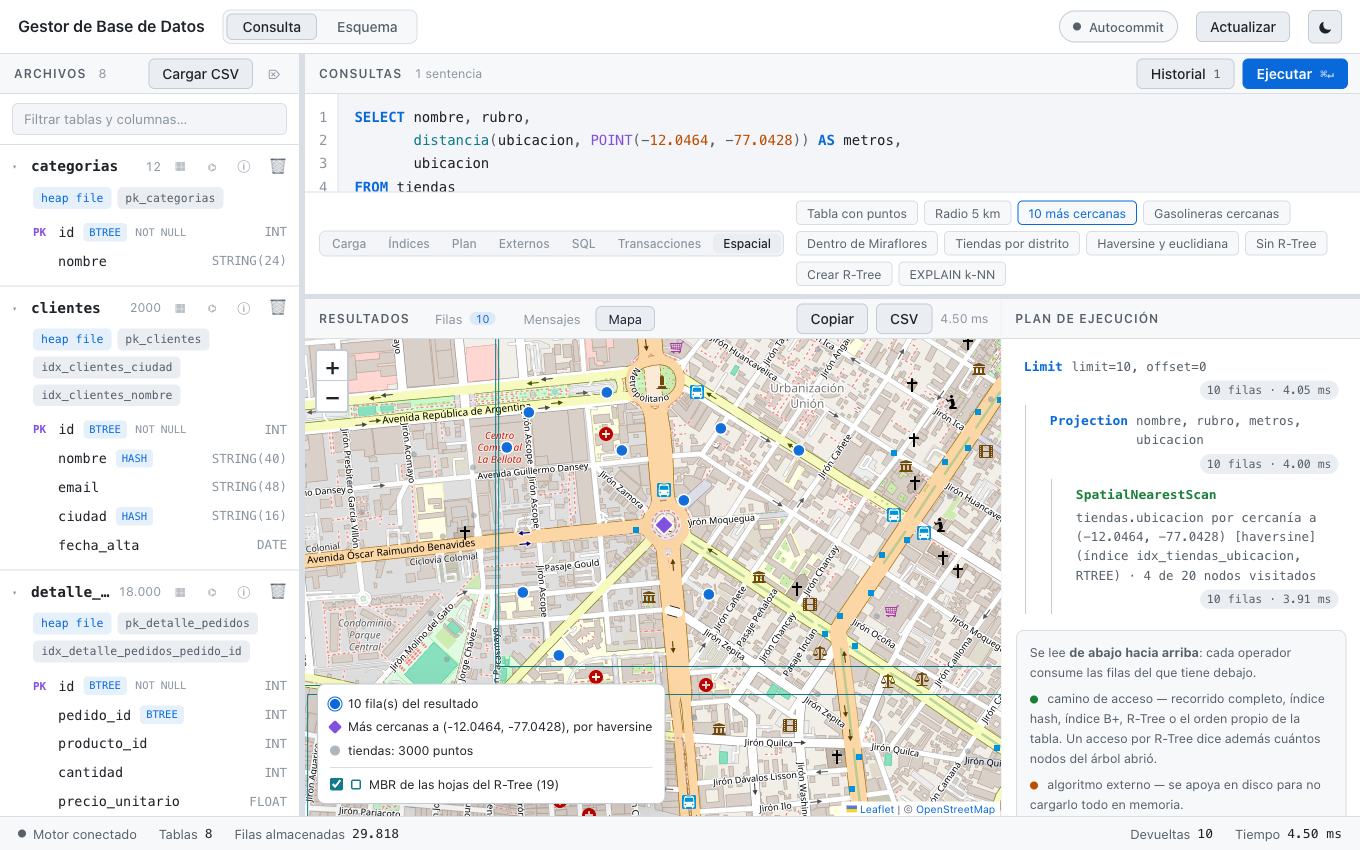
\includegraphics[width=0.94\textwidth]{figuras/interfaz.png}
  \caption{La interfaz tras pedir las 10 tiendas más cercanas a un punto. A la izquierda, los
           archivos con su organización y sus índices; arriba, el editor SQL con los atajos de
           ejemplo; en el centro, el resultado sobre el mapa, con los rectángulos (MBR) de las
           hojas del R-Tree; a la derecha, el plan de ejecución, que usó el índice y abrió 4
           de sus 20 nodos.}
  \label{fig:interfaz}
\end{figure}
